\documentclass[addpoints,spanish, 12pt,a4paper,cancelspace]{./include/gexam}

 %%%%%%%%%%%%%%%%%%%%%%%%%%%
 \renewcommand{\documentName} { Sistema de coordenadas cartesianos }
 \renewcommand{\documentContent} { \phantom{ } } 
 \renewcommand{\waterMark} { Modelo 8 } 

 % Configuración del documento.
 \renewcommand{\schoolSubject} { Examen Matemáticas 2º ESO  }
\renewcommand{\school} { IES José de Churriguera  }
\renewcommand{\academicPeriod} { Curso 2022/2023 }

\renewcommand{\autor} { Andrés Giménez Muñoz }
\renewcommand{\emailAuthor} { andresprofemates@outlook.es }
\renewcommand{\autorSing}{ Profesor: Andrés } 
 %%%%%%%%%%%%%%%%%%%%%%%%%%%
 
\renewcommand\subpartlabel{\thesubpart}
\renewcommand\subpartshook{\renewcommand\makelabel[1]{##1\hfil }} 
 
 %%%%%%%%%%%%%%%%%%%%%%%%%%%
 % Exam configuration
 %\pointsdroppedatright   %% No mostrar la puntuación
 \pointsinrightmargin{} % Para poner las puntuaciones a la derecha. Se puede cambiar. Si se comenta, sale a la izquierda.
 \extrawidth{-1.5cm} %Un poquito más de margen por si ponemos textos largos.
 \marginpointname{ \emph{\points}}
 
 %% Si se comenta no aparecerán los espacios de la solución.
 %\nocancelspace
 
 %% Puntuación a la izquierda.
%  \nopointsinrightmargin 

 %% Esto es de la clase exam. Si dejamos sin comentar \printanswers, se mostraran las soluciones. 
 %% Si la comentamos y dejamos sin comentar \noprintanswers, pues no se muestran las soluciones.
 % \printanswers
 %\noprintanswers
 
 %%%%%%%%%%%%%%%%%%%%%%%%%%%
 
 \begin{document}
 
%  \StudentData{}
%  \GradeTableHeader{}
 
 \justifying

% \begin{center}
%     \fbox{\fbox{\parbox{6.5in}{             
%                 \begin{itemize}
%                     \item Deben aparecer todas las operaciones, no vale solo con indicar el resultado.
%                     \item Se podrán quitar hasta cinco décimas por falta de claridad o rigor en el desarrollo de las respuestas o por una mala presentación.
%                     \item Se valorará que se indiquen las cuentas en línea, realizando las operaciones en el margen.
%                     \item No se puede utilizar la calculadora.
%                 \end{itemize}
%             }}}
% \end{center}
 
 \begin{questions}
    
    %% Gato
    \question Dibuja los puntos en el orden en el que aparece y únelos con segmentos de línea. \\
    \small

    Trazo 1: $(-14, 15)$ $(-8, 6)$ $(-6, 5)$ $(-3, 5)$ $(-3, 4)$ $(-7, 2)$ $(-7, -1)$ $(-13, -6)$ $(-13, -9)$ $(-12, -6)$ $(-13, -9)$ $(-13, -10)$ $(-12, -9)$ $(-12, -7)$ $(-11, -6)$ $(-10, -6)$ 
    $(-10, -7)$ $(-11, -9)$ $(-9, -7)$ $(-9,-6)$ $(-10, -5)$ $(-9, -4)$ $(-7, -4)$

    Trazo 2: $(-7, -1)$ $(-7, -7)$ $(-8, -11)$ $(-8, -14)$ $(-12, -17)$ $(-10, -18)$ $(-7, -17)$ $(-6, -15)$ $(-7, -17)$ $(-6, -18)$ $(-5, -18)$ $(-4, -17)$ $(-4, -15)$ $(-4, -17)$ $(-4, -17)$ 
    $(-4, -15)$ $(-4, -17)$ $(-1, -17)$ $(-1, -16)$ $(-2, -14)$ $(-3, -12)$ $(-3, -10)$ $(-2, -8)$ $(2, -12)$ $(3, -14)$ $(3, -18)$ $(5, -19)$ $(5, -17)$ $(5, -19)$ $(6, -20)$ $(8, -20)$ $(9, -19)$ 
    $(9, -17)$ $(9, -19)$ $(13, -19)$ $(11, -17)$ $(13, -19)$ $(14, -18)$ $(11, -15)$
    
    Trazo 3: $(11, -15)$ $(9, -14)$ $(7, -11)$ $(4, -6)$ $(3, -4)$ $(6, 0)$ $(6, 1)$ $(9, -2)$ $(9, -3)$ $(11, -5)$ $(8, -7)$ $(8, -9)$ $(9, -9)$ $(9, -8)$ $(10, -7)$ $(11, -7)$ $(10, -10)$ $(11, -9)$ 
    $(12, -7)$ $(12, -9)$ $(11, -11)$ $(13, -9)$ $(13, -8)$ $(13, -11)$ $(14, -10)$ $(14, -6)$ $(12, -3)$ $(11, -1)$ $(8, 3)$ $(6, 4)$ $(3, 4)$ $(2, 6)$ $(4, 7)$ $(6, 10)$ $(7, 15)$ $(7, 16)$
    
    Trazo 4: $(7, 16)$ $(6, 16)$ $(6, 17)$ $(5, 18)$ $(4, 18)$ $(4, 14)$ $(4, 19)$ $(1, 19)$ $(0, 18)$ $(0, 15)$ $(0, 20)$ $(-3, 20)$ $(-4, 18)$ $(-4, 16)$ $(-4, 19)$ $(-7, 18)$ $(-5, 13)$ $(-7, 18)$ 
    $(-8, 18)$ $(-7, 19)$ $(-9, 19)$ $(-9, 18)$ $(-10, 18)$ $(-11, 17)$ $(-11, 16)$ $(-10, 14)$ $(-11, 16)$ $(-12, 16)$ $(-14, 15)$
    
    Trazo 5: $(-9, 9)$ $(-8, 8)$ $(-7, 8)$ $(-6, 9)$ $(-7, 10)$ $(-8, 10)$ $(-9, 9)$
    
    Trazo 6: $(-1, 9)$ $(1, 9)$ $(2, 10)$ $(1, 11)$ $(-1, 11)$ $(-2, 10)$ $(-1, 9)$
    
    Trazo 7: $(-5, 6)$ $(-3, 6)$ $(0, 7)$
    
    \normalsize

    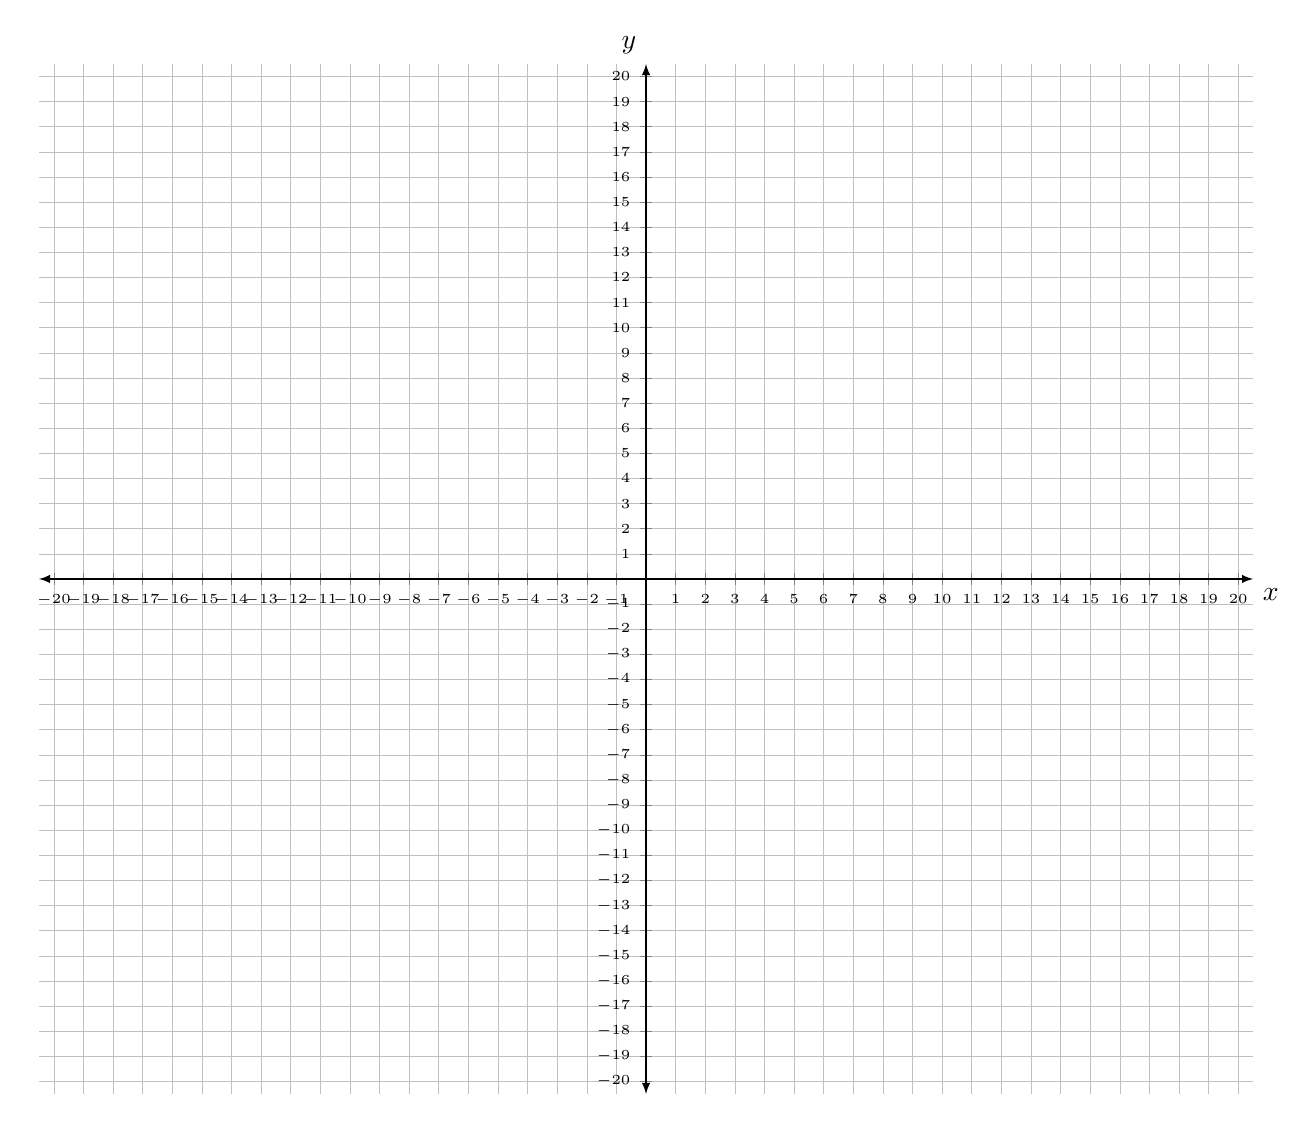
\begin{tikzpicture}[scale=1]
        \begin{axis}[
            axis x line=center,
            axis y line=center,
            xlabel = {$x$},
            ylabel = {$y$},
            xmin=-20,xmax=20,
            ymin=-20,ymax=20,
            xtick distance=1, 
            ytick distance=1, 
            grid=both,
            grid style={line width=.1pt, draw=gray!10},
            major grid style={line width=.2pt,draw=gray!50},
            axis lines=middle,
            axis line style={<->},
            minor tick num=0,
            enlargelimits={abs=0.5},
            axis line style={latex-latex},
            ticklabel style={font=\tiny},
            % ticklabel style={font=\tiny,fill=white},
            % xlabel style={at={(ticklabel* cs:1)},anchor=north west},
            % ylabel style={at={(ticklabel* cs:1$)},anchor=south west},
            xlabel style={below right},
            ylabel style={above left},
            width=17cm,
        ]
        
        \end{axis}

    \end{tikzpicture}

\end{questions}
 
\end{document}